

%Tähän voisi laittaa kuvan komponenttien asemmoitumisesta toisiinsa.
\subsubsection{Asiakaslaite}
Asiakaslaite (user equipment) on yleisnimitys reunan tai pilven palveluita kuluttavalla laitteelle.
Asiakaslaite käsitettä ei ole rajattu mihinkään tiettyihin laitteisiin ja asiakaslaite voikin olla esimerkiksi älypuhelin, älylasit tai verkkoyhteydellä varustettu auto. 
Asiakaslaitteiden yhdistävänä tekijänä on siis jonkinlainen yhteys reuna- tai pilvipalveluihin. Yleisesti asiakaslaitteen käyttämä yhteys on tyypiltään langaton. 
Yksinkertaisuuden vuoksi tässä tutkielmassa asiakaslaitteen voi ajatella älypuhelimena, jollei toisin mainita.

Verkkohierarkkian näkökulmasta asiakaslaitteet ovat lehtisolmuja. Tämä tarkoittaa että asiakaslaitteet toimivat ainoastaan palveluiden kuluttajina eivätkä siis tarjoa itse palveluita. Myöskään kulutettavien palveluiden tyypillä ei ole juurikaan merkitystä, kun asiaa käsitellään infrastruktuuri- tai arkkitehtuuritasolla.

Konkreettinen esimerkki asiakaslaitteesta, joka hyödyntää reunapalvelua, voisi olla jokin ajoneuvo.
Ajoneuvolla on mobiiliyhteys reunapalveluun, jonka tarkoitus on välittää tietoa liikenteestä muille ajoneuvoille. Esimerkiksi tilanteessa jossa edellä on ruuhkaa, voitaisiin muille lähistöllä oleville ajoneuvoille välittää tieto tästä, jolloin voidaan valita jokin toinen reitti määränpäähän.

\begin{figure}[tb]
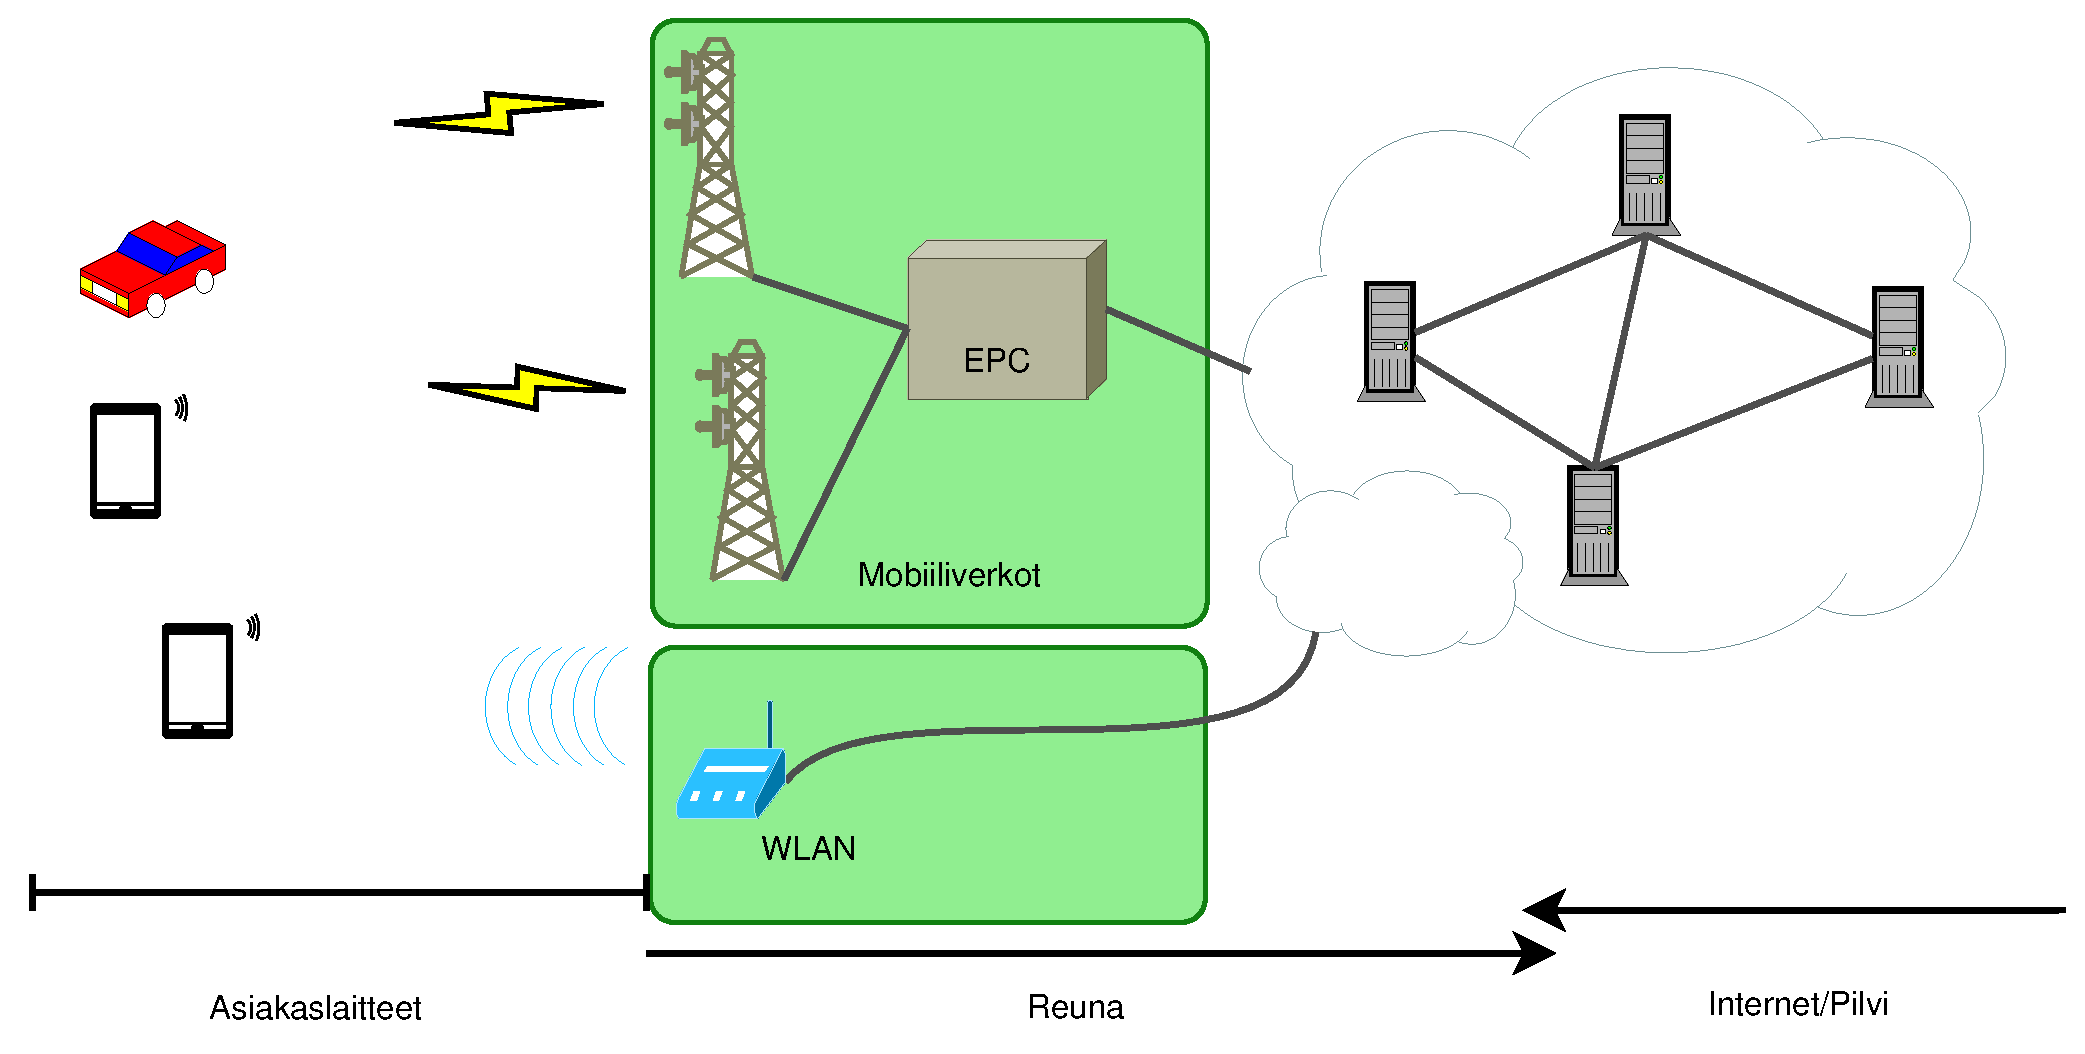
\includegraphics[width = \textwidth]{asiakasedgecloud.eps}
\caption{Asiakaslaitteiden, reunan ja pilven alueet} \label{fig:asiakasedgecloud}
\end{figure}

\subsubsection{Reuna} \label{reunatoimijat}
Reuna koostuu useista toiminnallisista entiteeteistä, jotka voidaan jakaa sekä fyysisiin että loogisiin kokonaisuuksiin. 
Tässä kappaleessa lähdetään liikkeelle määrittelemällä reuna-alue, joka edustaa reunan toimialuetta sekä reunaa yleisenä käsitteenä.
Tämän jälkeen määritellään reunasolmu, joka on reunajärjestelmän keskeisin fyysinen rakennuspalanen.
Lopuksi esitellään pääasiassa ohjelmallisella tasolla ilmenevät toimijat reuna-alusta ja reunasovellus.


\paragraph{Reuna-alue} 
Reunalla tai reuna-alueella viitataan alueeseen, joka alkaa asiakaslaitteen yhteyspisteestä. Tämä yhteyspiste voi olla esimerkiksi WLAN-tukiasema tai mobiiliverkon tukiasema. Tästä ensimmäisestä yhteyspisteestä reuna-alue laajenee kohti runkoverkkoa ja pilveä.
Kuvassa \ref{fig:asiakasedgecloud} reuna on kuvattu alkavan mobiiliverkon tukiasemasta tai WLAN-tukiasemasta ja laajenevan pilveä kohti.
Joidenkin näkemyksien mukaan myös asiakaslaitteet luetaan osaksi reunaa, tällöin niihin viitataan termillä reunalaite (edge device) \cite{garcia}.
Tämän tutkielman puitteissa asiakaslaitteet luetaan omaksi osakseen reuna-alueen toisella laidalla.
Reunan laajuudelle ei siis ole yksiselitteistä määritelmää, vaan termiä usein sovelletaan käytettävän kontekstin mukaan siten, että reuna-alue rajautuu kontekstissa esiintyvien toimijoiden mukaan edellä kuvatulle välille.
Esimerkiksi mobiiliverkon tukiasemien yhteyteen rakennettua reunajärjestelmää käsiteltäessä, reunalla tarkoitetaan ainoastaan reunajärjestelmän asiakaslaitteita palvelevien osien muodostamaa vyöhykettä. 
Kuten jo aiemmin mainittu, reunan keskeisenä etuna muihin palveluihin voidaan pitää reunapalveluiden ja asiakaslaitteen välisen viiveen vähäisyyttä.
Tämän pohjalta yleisenä nyrkkisääntönä reunalle voidaankin pitää verkkoyhteyksien viivettä suhteessa muuhun internettiin, koska reuna-alueella palveluiden viiveiden tulisi siis olla muuta internettiä nopeampia. Toisin sanoen reunan palveluiden tulisi sijaita lähempänä kuin pilvessä sijaitsevien palveluiden.

\begin{figure}[tb]
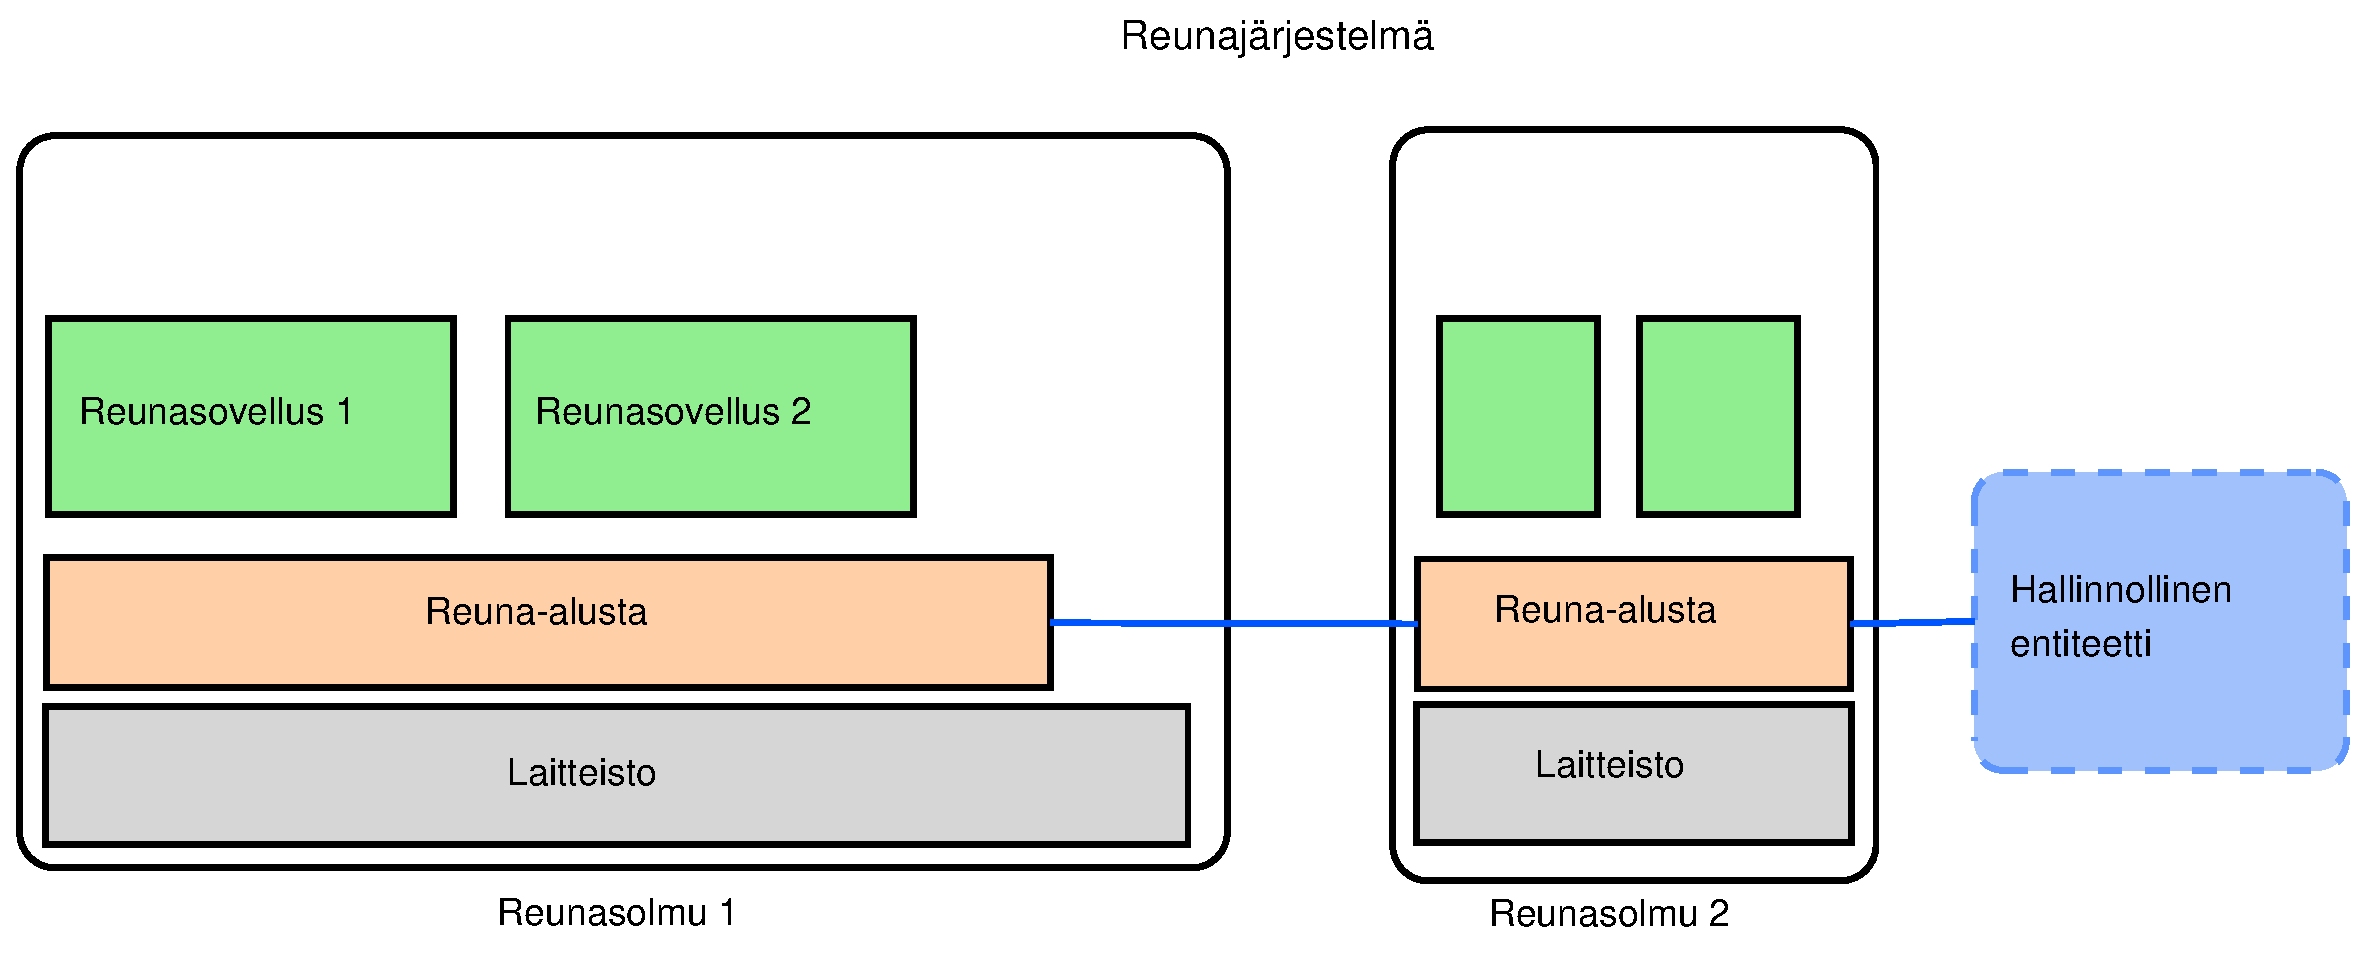
\includegraphics[width = \textwidth]{reunajarjestelma.eps}
\caption{Esimerkki reunajärjestelmän rakenteesta.} \label{fig:reunajarjestelma}
\end{figure}


\paragraph{Reunasolmu} 
Tämän tutkielman kontekstissa reunasolmulla (mobile edge host) tarkoitetaan yksittäistä reunalaskentaa tarjoavaa entiteettiä\cite{etsirefarch}.
Reunasolmu termillä viitataan reunasolmun fyysiseen laitteiston ja reunasolmun toiminnalliseen kokonaisuuteen.
Reunasolmu sisältää reunasovelluksien suorittamiseen tarvittavat resurssit, jotka ovat pääasiassa tavallisia palvelinresursseja kuten laskenta, tallennustila ja verkkoyhteydet.
Reunasolmu voi koostua esimerkiksi mobiilitukiaseman ja palvelinlaitteiston muodostamasta kokonaisuudesta. 
Reunasolmun toiminnallinen kokonaisuus sisältää erinäisiä toimintoja, joiden tehtävänä on mahdollistaa reunasovelluksien suorittaminen.
Tällaisia ovat muun muassa tietoliikenteen reitittäminen ja virtualisointialustan tarjoaminen, sekä sen hallinnointi.
Kuvassa \ref{fig:reunajarjestelma} on esitetty esimerkki reunasolmun sisällä olevista entiteeteistä. 
Seuraavaksi käsiteltävä reuna-alusta kattaa osan reunasolmun toiminnoista.

Kuten aiemmin mainittu, reunajärjestelmä koostuu joukosta reunasolmuja, jotka ovat maantieteellisesti hajautettuja.
Reunasolmut siis eroavat toisistaan vähintään sijainnin perusteella, mutta voivat erota myös käytettävissä olevien resurssien osalta. Resurssien osalta reunasolmu voi olla mitä tahansa vähäisillä laskenta ja tallennus resursseilla varustetun WiFi-tukiaseman ja kokonaisen palvelinklusterin väliltä.
Reunasolmun sijaintiin vaikuttaa käytössä oleva reuna-arkkitehtuuri.
%Kuten juuri mainittu, reunasolmujen sijaintiin vaikuttaa käytettävä reuna-arkkitehtuuri.
Reunan rakennetta ja reunasolmujen sijaintia käsitellään tarkemmin luvussa \ref{rakenne}.

\paragraph{Reuna-alusta}
Reuna-alusta (edge platform) on ohjelmistotason toimija. Se tarjoaa rajapinnan reunasovelluksien suorittamista varten \cite{etsirefarch}. Toisin sanoen se siis tarjoaa reunasovelluksille toimintaympäristön.
Reuna-alustan tehtävät eivät rajaudu ainoastaan yksittäiseen reunasolmuun, vaan sen lisäksi se hoitaa hallinnollisia tehtäviä kuten tietoliikenteen ohjausta. Lisäksi reuna-alustan tehtäviin voidaan lukea reunasovelluksia suorittaviin virtuaalikoneisiin liittyvät hallinnolliset toimet. Esimerkkinä reuna-alustan tehtävistä on kappaleessa \ref{livemigraatio} esiteltävä virtuaalikoneiden live migraatio reunasolmulta toiselle.
Reunasovelluksien lisäksi reuna-alusta voi itsessään tarjota palveluita, jotka eivät suoranaisesti ole reunasovelluksia vaan esimerkiksi nopea kommunikaatioväylä laitteelta-laitteelle (machine-to-machine), jota voi käyttää esimerkiksi ajoneuvojen väliseen kommunikointiin.
Koska reuna-alustan tehtäviin kuuluu hallinnolliset toimet, voidaan sen ajatella laajentuvan myös reunasolmun ulkopuolella sijaitseviin hallinnosta vastaaviin entiteetteihin.

\paragraph{Reunasovellus}
Reunasovelluksella (edge application) tarkoitetaan yksittäistä reunasolmulla suoritettava ohjelmistoa \cite{etsirefarch}, jonka kuluttajana voi toimia asiakaslaite tai toinen reunasovellus. Reunasovellukset tarjoavat \textit{reunapalveluita}.
Reunasovellus ei ota kantaa millaista palvelua sillä tuotetaan.

Reunasovelluksen tuottama reunapalvelun tyyppiä säätelee pääasiassa reuna-alusta sekä reunalaskennan liiketoimintamalli. Teoriassa mahdollisuudet ovat siis samat kuin pilvessä.
Esimerkkejä reunasovelluksen tuottaman palvelun tyypeistä ovat yhteiskäyttöinen tai käyttäjäkohtainen.
Esimerkki käyttäjäkohtaisesta reunasovelluksesta voisi olla käyttäjäkohtainen virtuaalikone johon käyttäjä voi ottaa etäyhteyden. Esimerkkinä yhteiskäyttöisestä reunasovelluksesta voisi olla pelipalvelin, jota voivat käyttää reunasolmun toimipiirissä olevat pelaajat.

Reunalaskenta ja reunasovellus viittaavat yleensä lähes samaan asiaan, mutta eri konteksteissa. 
Reunasovellus on ohjelmallinen entiteetti, joka sijaitsee reunajärjestelmän sisällä.
Reunalaskenta puolestaan viittaa reunajärjestelmän palveluiden käyttämiseen.

\paragraph{Reunalaskennan tyypit}

Reunalaskennan tyyppejä ovat etälaskenta (offloading) ja asiakaslaitetta tukevat erilaiset reunapalvelut.
Arkkitehtuuritasolla reunalaskennan tyyppiin ei oteta juurikaan kantaa. 
Jotkin suunnittelupäätökset voivat kuitenkin vaikuttaa siihen, millaisia reunalaskennan tyyppejä reunajärjestelmä lopulta tukee tai painottaa.
Etälaskennalla tarkoitetaan työyksiköiden (task) siirtämistä ulkoiselle laskentaa suorittavalle instanssille, joka palauttaa asiakaslaitteelle laskennan lopputuloksen. 
Reunajärjestelmässä suoritettava etälaskenta voidaan jakaa kahteen alakategoriaan: kokonaan reunalla suoritettaviin ja osittain reunalla suoritettaviin sovelluksiin\cite{mach17mobile}.
Kokonaan reunalla suoritettava laskenta on tyypiltään sellaista, että sitä ei voi jakaa useamman instanssin suoritettavaksi.
Tällöin vaihtoehdoksi jää suorittaa laskenta kokonaan paikallisesti tai siirtää se reunasolmulle suoritettavaksi.
Osittainen etälaskenta on vaihtoehto sovelluksille, jotka on mahdollista pilkkoa suoritettaviin työyksikköihin. 
Sovelluksen työyksiköt jakautuvat usein niihin jotka on mahdollista siirtää reunalle suoritettavaksi, sekä niihin joita ei ole mahdollista siirtää. 
Esimerkiksi valokuvan ottaminen on työyksikkö, jota ei ole mahdollista tehdä muuten kuin paikallisesti asiakaslaitteella \cite{mach17mobile}.
Päätös etälaskennan tekemistä on riippuvainen laskennan tavoitteesta. 
Tavoitteina voi olla esimerkiksi asiakaslaitteen virransäästön maksimointia tai laskennan suorituksen keston minimointia.
Reunapalvelu voi olla tyypiltään asiakaslaitteella suoritettavan sovelluksen toimintaa tukeva palvelu. Sen voi ajatella esimerkiksi pelipalvelimeksi, joka suorittaa pelimekaniikan simuloinnin ja asiakaslaitteelle jää tehtäväksi ainoastaan pelitilan visuaalinen esittäminen.  



\subsubsection{Pilvi}
%pilven alk peräinen määritelmä
Armbrust et al. esittävät artikkelissaan määritelmän pilvelle \cite{armbrust2010view}. 
Pilvellä viitataan sekä pilvessä tuotettaviin palveluihin, että itse tekniseen järjestelmään.
Järjestelmällä tarkoitetaan pilvialustaa, joka mahdollistaa palveluiden tuottamisen.
Artikkelin mukaan pilven tuottamisen yhtenä keskeisimpänä mahdollistajana on toiminut edullisille sijainneille rakennetut suuret palvelinsalit.
Toisin sanottuna pilvipalvelut tuotetaan palvelinsaleissa, jotka ovat keskitettyjä ja sijaitsevat kauempana asutuksesta. 

Keskeinen osa pilven paradigmaa on myös tapa, jolla palveluita tuotetaan.
Pilvialusta tarjoaa asiakkailleen mahdollisuuden skaalata palveluitaan näennäisesti äärettömyyksiin.
Tämän lisäksi aika, jossa käytössä olevien resurssien lisäys tai poisto voidaan tehdä, on huomattavasti lyhyempi verrattuna perinteiseen palvelinsaliin, jossa palvelun käyttäjä omistaisi itse palvelun tuottamiseen käytettävän laitteiston.
Tässä tutkielmassa pilvellä viitataan kuitenkin enemmänkin järjestelmän rakenteeseen ja sijaintiin, kuin palveluiden tuottamiseen käytettävään malliin.

Reunan ei ole tarkoitus korvata pilveä, vaan täydentää sitä. Pilven ja reunan välinen raja ei ole tarkka. Tässä tutkielmassa pilvellä tarkoitetaan suhteessa reunaa kauempana tuotettuja palveluita. Pilvi ulottuu verkon ytimestä kohti asiakaslaitetta ja saattaa olla osittain päällekkäin reunan kanssa. Vastoin kuin aiemmin mainittu reuna, joka lähestyy verkon ydintä asiakaslaitteen suunnasta. Kuvassa \ref{fig:asiakasedgecloud} esitetty reunan ja pilven laajenemissuunnat.

Pilven ja reunan väliin on ehdotettu vielä yhtä toteutusparadigmaa – sumua (fog computing).
Sumun tavoitteet ovat samankaltaisia kuin reunan. Sumun tavoitteita ovat muun muassa pienet viiveet, maantieteellisesti hajautettu rakenne ja langattomien laitteiden palvelu \cite{bonomi2012fog}. Sumun on tarkoitus olla hieman kuten pilvi, mutta hajautetumpana ja pilveen verrattuna huomattavasti lähempänä käyttäjää. Reunaan verrattuna sumu on hieman samankaltainen, mutta vietynä kauemmaksi verkon reunasta.
Sumua ei käsitellä tämän enempää tässä tutkielmassa, vaan keskitytään lähempänä reunaa sijaitsevaan laskentaan.



%Asiakaskohtaiselle reunainstanssille ei ole mitään vakiintunutta nimeä.
%Cloudlet on yksi ehdotettu toteutustekniikka tällaiselle asiakaskohtaiselle reunalla sijaitsevalle virtuaali-instanssille \cite{satya09}.

\subsection{Mobiiliverkko}
\begin{figure}[htb]
\includegraphics[scale=0.5]{EUTRAN}
\caption{Mobiiliverkon rakenne} \label{ekakuva}
\end{figure}

MEC ehdotuksia tarkasteltaessa, olemassa olevien mobiiliverkkojen arkkitehtuurit ovat keskeisessä asemassa. Useat reunalaskentaa käsittelevät ehdotukset on tarkoitettu integroitaviksi osaksi olemassa olevaa mobiiliverkkoarkkitehtuuria. 
Erityisesti asiakaslaitteiden ollessa mobiililaitteita ja mahdollisimman pieniä viiveitä tavoiteltaessa, reunalaskenta ratkaisujen integroiminen osaksi mobiiliverkkoa on väistämätöntä. Seuraavaksi käydään pääpiirteittäin läpi 4G mobiiliverkon arkkitehtuurin funktionaaliset osat.

Yksinkertaistettuna mobiiliverkko koostuu kahdesta osasta: radiorajapinnasta ja mobiilinverkon runkoverkosta (puhelinkeskuksesta?). 3GPP kehittämässä LTE standardissa radiorajapinnan sisältävä osuus on nimeltään E-UTRAN (Evolved UMTS Terrestrial Radio Access Network) ja runkoverkon osuus EPC (Evolved Packet Core).

E-UTRAN tehtävänä on toimia rajapintana asiakaslaitteen ja EPC:n välillä. Asiakaslaitteiden suuntaan yhteys on radiosignalointia ja yhtenä E-UTRAN tehtävänä onkin radioresurssien hallinointi. 
E-UTRAN sisältää verkon puolella pääasiallisena toimijana eNodeB tyyppisiä tukiasemia \cite{etsieutran}, myös muutamia poikkeustapauksia on, mutta ne jätetään käsittelemättä.
Tukiasema on asiakaslaitetta lähimpänä sijaitseva funktionaalinen verkon osa ja sen seurauksena se on houkutteleva kohde MEC ratkaisuille. Tukiasemaa voikin ajatella \textit{reunan} viimeisenä etappina ennen asiakaslaitetta. Tämä tutkielma käsittelee pääasiassa ratkaisuja, jotka keskittyvät LTE verkkoihin kohdistuvia ratkaisuja, joten tukiasemista puhuttaessa tarkoitetaan nimenomaan E-UTRAN mukaista eNodeB:tä. 

ENodeB:n tehtävänä on kommunikoida radioyhteyttä käyttäen asiakaslaitteen kanssa ja välittää molemminsuuntaista liikennettä EPC:n (Evolved packet core) suuntaan S1 rajapinnan kautta. eNodeB:t ovat myös yhteydessä toisiinsa X2 rajapintaa käyttäen. X2 rajapintaa käytetään tukiasemien väliseen kommunikointiin, joka sisältää handoverin yhteydessä tehtävää asiakaskontekstin siirtoa ja erinäisiä muita hallinnollisia toimintoja.  
Handoverin vaikutukset näkyvät myös MEC puolelle ja handoveria toimintaa käsitellään tarkemmin kappaleessa XYZ.

Mobiiliverkkojen tietoliikenne koostuu kahdesta eri tasosta: kontrollikerroksesta ja datakerroksesta.
Kontrollikerroksella on hallinnointiin liittyviä protokollia joiden tehtävänä on välittää esimerkiksi asiakaslaitteeseen liittyviä kontekstitietoja entiteetiltä toiselle. Datakerros puolestaan välittää IP liikennettä asiakkaan ja palveluiden välillä. 
EPC koostuu kolmesta alikomponentista jotka ovat MME (Mobility Management Entity), SGW (Serving Gateway) ja PGW (PDN gateway) \cite{etsilte}.
SGW:n eli palveluyhdyskäytävän tehtävänä on välittää datakerroksen liikennettä asiakaslaitteen ja ulkoisten palveluiden välillä. SGW on yhdistettynä PGW:hen, jonka tehtävänä on toimia IP tason reitittimenä EPC:n ja ulkoisen verkon välillä. PGW toimii asiakkaan ulkoverkon yhteyksien kiintopisteenä \cite{3gppepc}. MME on EPC:n hallinnollinen komponentti ja se toimii ainoastaan kontrollikerroksessa.

\subsection{Reunalaskenta-arkkitehtuuri}
%Määrittele mikä on reuna-arkkitehtuuri

%REUNA-ARKKITEHTUURI ON JOUKKO SUUNNITTELUPÄÄTÖKSIÄ!

Tässä tutkielmassa käsiteltävät arkkitehtuurit koostuvat oletusarkkitehtuurin (framework) tai suunnittelumallin (design model) tyylisistä arkkitehtuurikuvauksista. 
Oletusarkkitehtuuri jakaa järjestelmän jonkin tehtävän toteuttaviin kokonaisuuksiin, kuten komponentteihin ja moduuleihin \cite{ohark}. 
Suunnittelumallit puolestaan kuvaavat tarkemmin järjestelmän komponentteja sekä niiden toimintoja. Suunnittelumallit ovat kuitenkin ainoastaan osajoukko suunnittelupäätöksistä \cite{ohark2}, joten ne jättävät osan päätöksistä toteuttajalle. Lisäksi suunnittelumallit kuvaavat järjestelmää ainoastaan jollain tietyllä abstraktiotasolla ja koko järjestelmän kattavaan kuvaamiseen tarvittaisiin useita sisäkkäisiä ja hierarkkisia suunnittelumalleja \cite{ohark2}. 
Tässä tutkielmassa käsiteltävät reunalaskenta\hyp arkkitehtuurit ovat korkean tason luonnehdintoja järjestelmän ja sen osien toiminnasta jossain tietyssä ympäristössä.
Myöhemmin tutkielmassa esitettävä ETSI:n MEC spesifikaatio sisältää vaatimusmaisesti esitettyinä tarvittavat toimet, mutta eivät kuvaa niiden toteutusta.
Toisin sanoen tutkielmassa käsiteltävät arkkitehtuurit kattavat vain osajoukon kaikista järjestelmän toteuttamiseksi tarvittavista suunnittelupäätöksistä.
 
Reunalaskenta-arkkitehtuurissa toiminnalliset osat on jaettu loogisiin kokonaisuuksiin, eli tehtävien mukaan kasattuihin komponentteihin. Reunalaskenta\hyp arkkitehtuurit asettavat rajoitteita myös toimintojen fyysiselle sijoittumiselle, jolloin osa toimijoista on jaoteltu fyysisiin komponentteihin. Joskin kappaleessa \ref{nfv} esiteltävä NFV tekee toimintojen fyysisestä sijoittumisesta dynaamisempaa ja vähemmän laitteistoon sidonnaista. 
%Oletusarkkitehtuuria voidaan hyödyntää varsinaista toteutettavaa järjestelmää suunniteltaessa ja sovellusaluemallit kuvaavat järjestelmän osia suhteessa myös reunajärjestelmää ympäröiviin toimijoihin.
Kappaleessa \ref{reunatoimijat} käsiteltyjen reunaan liittyvien termien puitteissa, tässä tutkielmassa reunalaskenta-arkkitehtuurit keskittyvät reunasolmun ja reuna-alustan toiminnalliseen määrittelyyn. 
Tämän lisäksi reunajärjestelmää käsitellään alijärjestelmänä, eli osana suurempaa kokonaisjärjestelmää, joka koostuu muun muassa mobiiliverkosta.
Reunalaskenta\hyp arkkitehtuurit eivät siis tämän tutkielman puitteissa osa kantaa suoritettaviin reunasovelluksiin tai niiden toimintaan.

%Tämän tutkielman puitteissa arkkitehtuurilla tarkoitetaan reuna-alustan ja reunasolmujen muodostamaa järjestelmää. Reuna-alustan toiminnallisuuksia voisi eritellä vielä tarkemmin, etenkin reunasovelluksien hallinnan osalta. Cloudlet on konkreettinen toteutus reuna-alustan reunasovelluksia hallinnoivasta osasta, mutta se ei kata kuin yhden reunasolmun kerrallaan. 
%Tämän lisäksi olemassa on reunasolmujen välisestä hallinnasta vastaava kerros, tosin tämä kerros voi olla ulkoistettu erillisille hallinnolliselle toimijalle, jolloin hallinnollinen osa reuna-alustasta on varsinaisten reunasolmujen ulkopuolella. 

%Reunasovelluksien toimintaa ei käsitellä tarkemmin. Taxonomy paperissa on hyvä jaottelu erilaisista sovelluksista. Tämä aihepiiri laajenee sovelluksien jakamiseen osittain reunalla suoritettaviin (offloading) tai mobiilisovelluksen suoritusta tukeviin sovelluksiin. 

